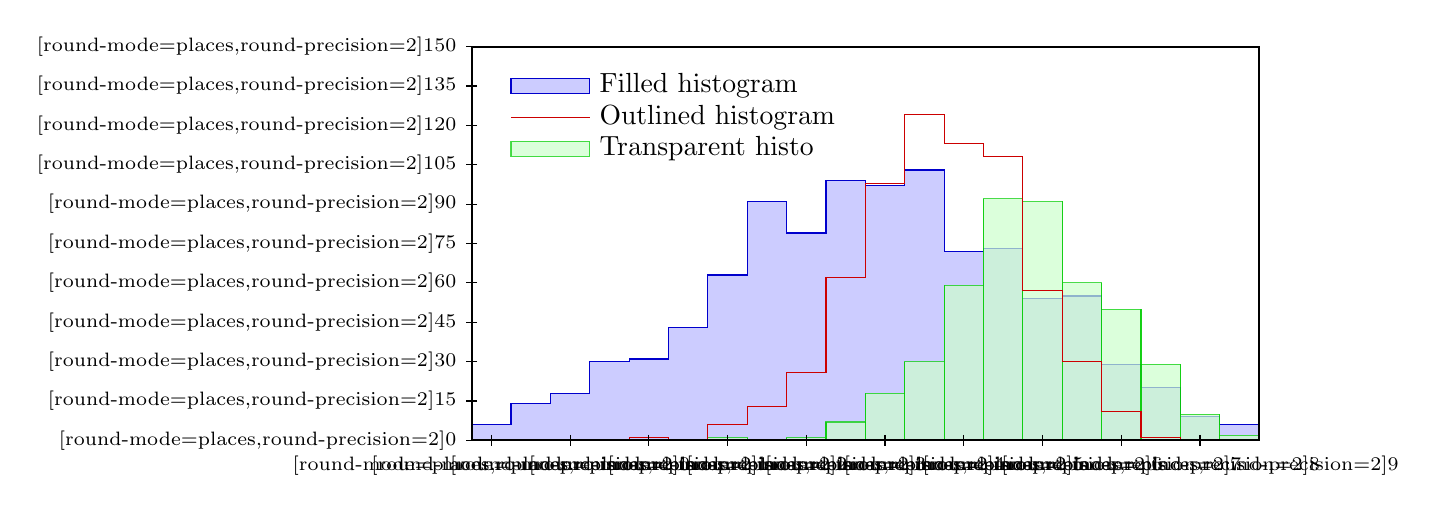
\begin{tikzpicture}[]
\begin{scope}[]
\clip (0,0) rectangle (10,5);
\begin{scope}[shift={(0.0,0.0)}]
\pgfsetxvec{\pgfpoint{1.0cm}{0cm}}
\pgfsetyvec{\pgfpoint{0cm}{0.033333335cm}}
\begin{scope}[draw=blue!80!black,fill=blue!20]
\pgfpathmoveto{ \pgfqpointxy {10.0} {0.0}}
\pgfpathlineto{ \pgfqpointxy {10.0} {6.0}}
\pgfpathlineto{ \pgfqpointxy {9.5} {6.0}}
\pgfpathlineto{ \pgfqpointxy {9.5} {9.0}}
\pgfpathlineto{ \pgfqpointxy {9.0} {9.0}}
\pgfpathlineto{ \pgfqpointxy {9.0} {20.0}}
\pgfpathlineto{ \pgfqpointxy {8.5} {20.0}}
\pgfpathlineto{ \pgfqpointxy {8.5} {29.0}}
\pgfpathlineto{ \pgfqpointxy {8.0} {29.0}}
\pgfpathlineto{ \pgfqpointxy {8.0} {55.0}}
\pgfpathlineto{ \pgfqpointxy {7.5} {55.0}}
\pgfpathlineto{ \pgfqpointxy {7.5} {54.0}}
\pgfpathlineto{ \pgfqpointxy {7.0} {54.0}}
\pgfpathlineto{ \pgfqpointxy {7.0} {73.0}}
\pgfpathlineto{ \pgfqpointxy {6.5} {73.0}}
\pgfpathlineto{ \pgfqpointxy {6.5} {72.0}}
\pgfpathlineto{ \pgfqpointxy {6.0} {72.0}}
\pgfpathlineto{ \pgfqpointxy {6.0} {103.0}}
\pgfpathlineto{ \pgfqpointxy {5.5} {103.0}}
\pgfpathlineto{ \pgfqpointxy {5.5} {97.0}}
\pgfpathlineto{ \pgfqpointxy {5.0} {97.0}}
\pgfpathlineto{ \pgfqpointxy {5.0} {99.0}}
\pgfpathlineto{ \pgfqpointxy {4.5} {99.0}}
\pgfpathlineto{ \pgfqpointxy {4.5} {79.0}}
\pgfpathlineto{ \pgfqpointxy {4.0} {79.0}}
\pgfpathlineto{ \pgfqpointxy {4.0} {91.0}}
\pgfpathlineto{ \pgfqpointxy {3.5} {91.0}}
\pgfpathlineto{ \pgfqpointxy {3.5} {63.0}}
\pgfpathlineto{ \pgfqpointxy {3.0} {63.0}}
\pgfpathlineto{ \pgfqpointxy {3.0} {43.0}}
\pgfpathlineto{ \pgfqpointxy {2.5} {43.0}}
\pgfpathlineto{ \pgfqpointxy {2.5} {31.0}}
\pgfpathlineto{ \pgfqpointxy {2.0} {31.0}}
\pgfpathlineto{ \pgfqpointxy {2.0} {30.0}}
\pgfpathlineto{ \pgfqpointxy {1.5} {30.0}}
\pgfpathlineto{ \pgfqpointxy {1.5} {18.0}}
\pgfpathlineto{ \pgfqpointxy {1.0} {18.0}}
\pgfpathlineto{ \pgfqpointxy {1.0} {14.0}}
\pgfpathlineto{ \pgfqpointxy {0.5} {14.0}}
\pgfpathlineto{ \pgfqpointxy {0.5} {6.0}}
\pgfpathlineto{ \pgfqpointxy {0.0} {6.0}}
\pgfpathlineto{ \pgfqpointxy {0.0} {0.0}}
\pgfusepath{ fill,stroke }
\end{scope}
\begin{scope}[opacity=0.7,draw=green!80!black,fill=green!20]
\pgfpathmoveto{ \pgfqpointxy {10.0} {0.0}}
\pgfpathlineto{ \pgfqpointxy {10.0} {2.0}}
\pgfpathlineto{ \pgfqpointxy {9.5} {2.0}}
\pgfpathlineto{ \pgfqpointxy {9.5} {10.0}}
\pgfpathlineto{ \pgfqpointxy {9.0} {10.0}}
\pgfpathlineto{ \pgfqpointxy {9.0} {29.0}}
\pgfpathlineto{ \pgfqpointxy {8.5} {29.0}}
\pgfpathlineto{ \pgfqpointxy {8.5} {50.0}}
\pgfpathlineto{ \pgfqpointxy {8.0} {50.0}}
\pgfpathlineto{ \pgfqpointxy {8.0} {60.0}}
\pgfpathlineto{ \pgfqpointxy {7.5} {60.0}}
\pgfpathlineto{ \pgfqpointxy {7.5} {91.0}}
\pgfpathlineto{ \pgfqpointxy {7.0} {91.0}}
\pgfpathlineto{ \pgfqpointxy {7.0} {92.0}}
\pgfpathlineto{ \pgfqpointxy {6.5} {92.0}}
\pgfpathlineto{ \pgfqpointxy {6.5} {59.0}}
\pgfpathlineto{ \pgfqpointxy {6.0} {59.0}}
\pgfpathlineto{ \pgfqpointxy {6.0} {30.0}}
\pgfpathlineto{ \pgfqpointxy {5.5} {30.0}}
\pgfpathlineto{ \pgfqpointxy {5.5} {18.0}}
\pgfpathlineto{ \pgfqpointxy {5.0} {18.0}}
\pgfpathlineto{ \pgfqpointxy {5.0} {7.0}}
\pgfpathlineto{ \pgfqpointxy {4.5} {7.0}}
\pgfpathlineto{ \pgfqpointxy {4.5} {1.0}}
\pgfpathlineto{ \pgfqpointxy {4.0} {1.0}}
\pgfpathlineto{ \pgfqpointxy {4.0} {0.0}}
\pgfpathlineto{ \pgfqpointxy {3.5} {0.0}}
\pgfpathlineto{ \pgfqpointxy {3.5} {1.0}}
\pgfpathlineto{ \pgfqpointxy {3.0} {1.0}}
\pgfpathlineto{ \pgfqpointxy {3.0} {0.0}}
\pgfpathlineto{ \pgfqpointxy {2.5} {0.0}}
\pgfpathlineto{ \pgfqpointxy {2.5} {0.0}}
\pgfpathlineto{ \pgfqpointxy {2.0} {0.0}}
\pgfpathlineto{ \pgfqpointxy {2.0} {0.0}}
\pgfpathlineto{ \pgfqpointxy {1.5} {0.0}}
\pgfpathlineto{ \pgfqpointxy {1.5} {0.0}}
\pgfpathlineto{ \pgfqpointxy {1.0} {0.0}}
\pgfpathlineto{ \pgfqpointxy {1.0} {0.0}}
\pgfpathlineto{ \pgfqpointxy {0.5} {0.0}}
\pgfpathlineto{ \pgfqpointxy {0.5} {0.0}}
\pgfpathlineto{ \pgfqpointxy {0.0} {0.0}}
\pgfpathlineto{ \pgfqpointxy {0.0} {0.0}}
\pgfusepath{ fill,stroke }
\end{scope}
\begin{scope}[opacity=0.7,draw=green!80!black,fill=green!20]
\pgfpathmoveto{ \pgfqpointxy {10.0} {0.0}}
\pgfpathlineto{ \pgfqpointxy {10.0} {0.0}}
\pgfusepath{ stroke }
\end{scope}
\begin{scope}[opacity=0.7,draw=green!80!black,fill=green!20]
\pgfpathmoveto{ \pgfqpointxy {10.0} {2.0}}
\pgfpathlineto{ \pgfqpointxy {10.0} {0.0}}
\pgfusepath{ stroke }
\end{scope}
\begin{scope}[opacity=0.7,draw=green!80!black,fill=green!20]
\pgfpathmoveto{ \pgfqpointxy {9.5} {2.0}}
\pgfpathlineto{ \pgfqpointxy {9.5} {0.0}}
\pgfusepath{ stroke }
\end{scope}
\begin{scope}[opacity=0.7,draw=green!80!black,fill=green!20]
\pgfpathmoveto{ \pgfqpointxy {9.5} {10.0}}
\pgfpathlineto{ \pgfqpointxy {9.5} {0.0}}
\pgfusepath{ stroke }
\end{scope}
\begin{scope}[opacity=0.7,draw=green!80!black,fill=green!20]
\pgfpathmoveto{ \pgfqpointxy {9.0} {10.0}}
\pgfpathlineto{ \pgfqpointxy {9.0} {0.0}}
\pgfusepath{ stroke }
\end{scope}
\begin{scope}[opacity=0.7,draw=green!80!black,fill=green!20]
\pgfpathmoveto{ \pgfqpointxy {9.0} {29.0}}
\pgfpathlineto{ \pgfqpointxy {9.0} {0.0}}
\pgfusepath{ stroke }
\end{scope}
\begin{scope}[opacity=0.7,draw=green!80!black,fill=green!20]
\pgfpathmoveto{ \pgfqpointxy {8.5} {29.0}}
\pgfpathlineto{ \pgfqpointxy {8.5} {0.0}}
\pgfusepath{ stroke }
\end{scope}
\begin{scope}[opacity=0.7,draw=green!80!black,fill=green!20]
\pgfpathmoveto{ \pgfqpointxy {8.5} {50.0}}
\pgfpathlineto{ \pgfqpointxy {8.5} {0.0}}
\pgfusepath{ stroke }
\end{scope}
\begin{scope}[opacity=0.7,draw=green!80!black,fill=green!20]
\pgfpathmoveto{ \pgfqpointxy {8.0} {50.0}}
\pgfpathlineto{ \pgfqpointxy {8.0} {0.0}}
\pgfusepath{ stroke }
\end{scope}
\begin{scope}[opacity=0.7,draw=green!80!black,fill=green!20]
\pgfpathmoveto{ \pgfqpointxy {8.0} {60.0}}
\pgfpathlineto{ \pgfqpointxy {8.0} {0.0}}
\pgfusepath{ stroke }
\end{scope}
\begin{scope}[opacity=0.7,draw=green!80!black,fill=green!20]
\pgfpathmoveto{ \pgfqpointxy {7.5} {60.0}}
\pgfpathlineto{ \pgfqpointxy {7.5} {0.0}}
\pgfusepath{ stroke }
\end{scope}
\begin{scope}[opacity=0.7,draw=green!80!black,fill=green!20]
\pgfpathmoveto{ \pgfqpointxy {7.5} {91.0}}
\pgfpathlineto{ \pgfqpointxy {7.5} {0.0}}
\pgfusepath{ stroke }
\end{scope}
\begin{scope}[opacity=0.7,draw=green!80!black,fill=green!20]
\pgfpathmoveto{ \pgfqpointxy {7.0} {91.0}}
\pgfpathlineto{ \pgfqpointxy {7.0} {0.0}}
\pgfusepath{ stroke }
\end{scope}
\begin{scope}[opacity=0.7,draw=green!80!black,fill=green!20]
\pgfpathmoveto{ \pgfqpointxy {7.0} {92.0}}
\pgfpathlineto{ \pgfqpointxy {7.0} {0.0}}
\pgfusepath{ stroke }
\end{scope}
\begin{scope}[opacity=0.7,draw=green!80!black,fill=green!20]
\pgfpathmoveto{ \pgfqpointxy {6.5} {92.0}}
\pgfpathlineto{ \pgfqpointxy {6.5} {0.0}}
\pgfusepath{ stroke }
\end{scope}
\begin{scope}[opacity=0.7,draw=green!80!black,fill=green!20]
\pgfpathmoveto{ \pgfqpointxy {6.5} {59.0}}
\pgfpathlineto{ \pgfqpointxy {6.5} {0.0}}
\pgfusepath{ stroke }
\end{scope}
\begin{scope}[opacity=0.7,draw=green!80!black,fill=green!20]
\pgfpathmoveto{ \pgfqpointxy {6.0} {59.0}}
\pgfpathlineto{ \pgfqpointxy {6.0} {0.0}}
\pgfusepath{ stroke }
\end{scope}
\begin{scope}[opacity=0.7,draw=green!80!black,fill=green!20]
\pgfpathmoveto{ \pgfqpointxy {6.0} {30.0}}
\pgfpathlineto{ \pgfqpointxy {6.0} {0.0}}
\pgfusepath{ stroke }
\end{scope}
\begin{scope}[opacity=0.7,draw=green!80!black,fill=green!20]
\pgfpathmoveto{ \pgfqpointxy {5.5} {30.0}}
\pgfpathlineto{ \pgfqpointxy {5.5} {0.0}}
\pgfusepath{ stroke }
\end{scope}
\begin{scope}[opacity=0.7,draw=green!80!black,fill=green!20]
\pgfpathmoveto{ \pgfqpointxy {5.5} {18.0}}
\pgfpathlineto{ \pgfqpointxy {5.5} {0.0}}
\pgfusepath{ stroke }
\end{scope}
\begin{scope}[opacity=0.7,draw=green!80!black,fill=green!20]
\pgfpathmoveto{ \pgfqpointxy {5.0} {18.0}}
\pgfpathlineto{ \pgfqpointxy {5.0} {0.0}}
\pgfusepath{ stroke }
\end{scope}
\begin{scope}[opacity=0.7,draw=green!80!black,fill=green!20]
\pgfpathmoveto{ \pgfqpointxy {5.0} {7.0}}
\pgfpathlineto{ \pgfqpointxy {5.0} {0.0}}
\pgfusepath{ stroke }
\end{scope}
\begin{scope}[opacity=0.7,draw=green!80!black,fill=green!20]
\pgfpathmoveto{ \pgfqpointxy {4.5} {7.0}}
\pgfpathlineto{ \pgfqpointxy {4.5} {0.0}}
\pgfusepath{ stroke }
\end{scope}
\begin{scope}[opacity=0.7,draw=green!80!black,fill=green!20]
\pgfpathmoveto{ \pgfqpointxy {4.5} {1.0}}
\pgfpathlineto{ \pgfqpointxy {4.5} {0.0}}
\pgfusepath{ stroke }
\end{scope}
\begin{scope}[opacity=0.7,draw=green!80!black,fill=green!20]
\pgfpathmoveto{ \pgfqpointxy {4.0} {1.0}}
\pgfpathlineto{ \pgfqpointxy {4.0} {0.0}}
\pgfusepath{ stroke }
\end{scope}
\begin{scope}[opacity=0.7,draw=green!80!black,fill=green!20]
\pgfpathmoveto{ \pgfqpointxy {4.0} {0.0}}
\pgfpathlineto{ \pgfqpointxy {4.0} {0.0}}
\pgfusepath{ stroke }
\end{scope}
\begin{scope}[opacity=0.7,draw=green!80!black,fill=green!20]
\pgfpathmoveto{ \pgfqpointxy {3.5} {0.0}}
\pgfpathlineto{ \pgfqpointxy {3.5} {0.0}}
\pgfusepath{ stroke }
\end{scope}
\begin{scope}[opacity=0.7,draw=green!80!black,fill=green!20]
\pgfpathmoveto{ \pgfqpointxy {3.5} {1.0}}
\pgfpathlineto{ \pgfqpointxy {3.5} {0.0}}
\pgfusepath{ stroke }
\end{scope}
\begin{scope}[opacity=0.7,draw=green!80!black,fill=green!20]
\pgfpathmoveto{ \pgfqpointxy {3.0} {1.0}}
\pgfpathlineto{ \pgfqpointxy {3.0} {0.0}}
\pgfusepath{ stroke }
\end{scope}
\begin{scope}[opacity=0.7,draw=green!80!black,fill=green!20]
\pgfpathmoveto{ \pgfqpointxy {3.0} {0.0}}
\pgfpathlineto{ \pgfqpointxy {3.0} {0.0}}
\pgfusepath{ stroke }
\end{scope}
\begin{scope}[opacity=0.7,draw=green!80!black,fill=green!20]
\pgfpathmoveto{ \pgfqpointxy {2.5} {0.0}}
\pgfpathlineto{ \pgfqpointxy {2.5} {0.0}}
\pgfusepath{ stroke }
\end{scope}
\begin{scope}[opacity=0.7,draw=green!80!black,fill=green!20]
\pgfpathmoveto{ \pgfqpointxy {2.5} {0.0}}
\pgfpathlineto{ \pgfqpointxy {2.5} {0.0}}
\pgfusepath{ stroke }
\end{scope}
\begin{scope}[opacity=0.7,draw=green!80!black,fill=green!20]
\pgfpathmoveto{ \pgfqpointxy {2.0} {0.0}}
\pgfpathlineto{ \pgfqpointxy {2.0} {0.0}}
\pgfusepath{ stroke }
\end{scope}
\begin{scope}[opacity=0.7,draw=green!80!black,fill=green!20]
\pgfpathmoveto{ \pgfqpointxy {2.0} {0.0}}
\pgfpathlineto{ \pgfqpointxy {2.0} {0.0}}
\pgfusepath{ stroke }
\end{scope}
\begin{scope}[opacity=0.7,draw=green!80!black,fill=green!20]
\pgfpathmoveto{ \pgfqpointxy {1.5} {0.0}}
\pgfpathlineto{ \pgfqpointxy {1.5} {0.0}}
\pgfusepath{ stroke }
\end{scope}
\begin{scope}[opacity=0.7,draw=green!80!black,fill=green!20]
\pgfpathmoveto{ \pgfqpointxy {1.5} {0.0}}
\pgfpathlineto{ \pgfqpointxy {1.5} {0.0}}
\pgfusepath{ stroke }
\end{scope}
\begin{scope}[opacity=0.7,draw=green!80!black,fill=green!20]
\pgfpathmoveto{ \pgfqpointxy {1.0} {0.0}}
\pgfpathlineto{ \pgfqpointxy {1.0} {0.0}}
\pgfusepath{ stroke }
\end{scope}
\begin{scope}[opacity=0.7,draw=green!80!black,fill=green!20]
\pgfpathmoveto{ \pgfqpointxy {1.0} {0.0}}
\pgfpathlineto{ \pgfqpointxy {1.0} {0.0}}
\pgfusepath{ stroke }
\end{scope}
\begin{scope}[opacity=0.7,draw=green!80!black,fill=green!20]
\pgfpathmoveto{ \pgfqpointxy {0.5} {0.0}}
\pgfpathlineto{ \pgfqpointxy {0.5} {0.0}}
\pgfusepath{ stroke }
\end{scope}
\begin{scope}[opacity=0.7,draw=green!80!black,fill=green!20]
\pgfpathmoveto{ \pgfqpointxy {0.5} {0.0}}
\pgfpathlineto{ \pgfqpointxy {0.5} {0.0}}
\pgfusepath{ stroke }
\end{scope}
\begin{scope}[opacity=0.7,draw=green!80!black,fill=green!20]
\pgfpathmoveto{ \pgfqpointxy {0.0} {0.0}}
\pgfpathlineto{ \pgfqpointxy {0.0} {0.0}}
\pgfusepath{ stroke }
\end{scope}
\begin{scope}[opacity=0.7,draw=green!80!black,fill=green!20]
\pgfpathmoveto{ \pgfqpointxy {0.0} {0.0}}
\pgfpathlineto{ \pgfqpointxy {0.0} {0.0}}
\pgfusepath{ stroke }
\end{scope}
\begin{scope}[red!80!black]
\pgfpathmoveto{ \pgfqpointxy {10.0} {0.0}}
\pgfpathlineto{ \pgfqpointxy {10.0} {0.0}}
\pgfpathlineto{ \pgfqpointxy {9.5} {0.0}}
\pgfpathlineto{ \pgfqpointxy {9.5} {0.0}}
\pgfpathlineto{ \pgfqpointxy {9.0} {0.0}}
\pgfpathlineto{ \pgfqpointxy {9.0} {1.0}}
\pgfpathlineto{ \pgfqpointxy {8.5} {1.0}}
\pgfpathlineto{ \pgfqpointxy {8.5} {11.0}}
\pgfpathlineto{ \pgfqpointxy {8.0} {11.0}}
\pgfpathlineto{ \pgfqpointxy {8.0} {30.0}}
\pgfpathlineto{ \pgfqpointxy {7.5} {30.0}}
\pgfpathlineto{ \pgfqpointxy {7.5} {57.0}}
\pgfpathlineto{ \pgfqpointxy {7.0} {57.0}}
\pgfpathlineto{ \pgfqpointxy {7.0} {108.0}}
\pgfpathlineto{ \pgfqpointxy {6.5} {108.0}}
\pgfpathlineto{ \pgfqpointxy {6.5} {113.0}}
\pgfpathlineto{ \pgfqpointxy {6.0} {113.0}}
\pgfpathlineto{ \pgfqpointxy {6.0} {124.0}}
\pgfpathlineto{ \pgfqpointxy {5.5} {124.0}}
\pgfpathlineto{ \pgfqpointxy {5.5} {98.0}}
\pgfpathlineto{ \pgfqpointxy {5.0} {98.0}}
\pgfpathlineto{ \pgfqpointxy {5.0} {62.0}}
\pgfpathlineto{ \pgfqpointxy {4.5} {62.0}}
\pgfpathlineto{ \pgfqpointxy {4.5} {26.0}}
\pgfpathlineto{ \pgfqpointxy {4.0} {26.0}}
\pgfpathlineto{ \pgfqpointxy {4.0} {13.0}}
\pgfpathlineto{ \pgfqpointxy {3.5} {13.0}}
\pgfpathlineto{ \pgfqpointxy {3.5} {6.0}}
\pgfpathlineto{ \pgfqpointxy {3.0} {6.0}}
\pgfpathlineto{ \pgfqpointxy {3.0} {0.0}}
\pgfpathlineto{ \pgfqpointxy {2.5} {0.0}}
\pgfpathlineto{ \pgfqpointxy {2.5} {1.0}}
\pgfpathlineto{ \pgfqpointxy {2.0} {1.0}}
\pgfpathlineto{ \pgfqpointxy {2.0} {0.0}}
\pgfpathlineto{ \pgfqpointxy {1.5} {0.0}}
\pgfpathlineto{ \pgfqpointxy {1.5} {0.0}}
\pgfpathlineto{ \pgfqpointxy {1.0} {0.0}}
\pgfpathlineto{ \pgfqpointxy {1.0} {0.0}}
\pgfpathlineto{ \pgfqpointxy {0.5} {0.0}}
\pgfpathlineto{ \pgfqpointxy {0.5} {0.0}}
\pgfpathlineto{ \pgfqpointxy {0.0} {0.0}}
\pgfpathlineto{ \pgfqpointxy {0.0} {0.0}}
\pgfusepath{ stroke }
\end{scope}
\pgfsetxvec{\pgfpoint{1cm}{0cm}}
\pgfsetyvec{\pgfpoint{0cm}{1cm}}
\end{scope}
\end{scope}
\begin{scope}[shift={(0.0,0.0)}]
\pgfsetxvec{\pgfpoint{1.0cm}{0cm}}
\pgfsetyvec{\pgfpoint{0cm}{0.033333335cm}}
\begin{scope}[yshift=0cm]
\draw[] [shift={(0.25,0.0)}] (0pt,2pt) -- (-0pt,-2pt) node[below]{ \scriptsize{\num[round-mode=places,round-precision=2]{0}}};
\draw[] [shift={(1.25,0.0)}] (0pt,2pt) -- (-0pt,-2pt) node[below]{ \scriptsize{\num[round-mode=places,round-precision=2]{1}}};
\draw[] [shift={(2.25,0.0)}] (0pt,2pt) -- (-0pt,-2pt) node[below]{ \scriptsize{\num[round-mode=places,round-precision=2]{2}}};
\draw[] [shift={(3.25,0.0)}] (0pt,2pt) -- (-0pt,-2pt) node[below]{ \scriptsize{\num[round-mode=places,round-precision=2]{3}}};
\draw[] [shift={(4.25,0.0)}] (0pt,2pt) -- (-0pt,-2pt) node[below]{ \scriptsize{\num[round-mode=places,round-precision=2]{4}}};
\draw[] [shift={(5.25,0.0)}] (0pt,2pt) -- (-0pt,-2pt) node[below]{ \scriptsize{\num[round-mode=places,round-precision=2]{5}}};
\draw[] [shift={(6.25,0.0)}] (0pt,2pt) -- (-0pt,-2pt) node[below]{ \scriptsize{\num[round-mode=places,round-precision=2]{6}}};
\draw[] [shift={(7.25,0.0)}] (0pt,2pt) -- (-0pt,-2pt) node[below]{ \scriptsize{\num[round-mode=places,round-precision=2]{7}}};
\draw[] [shift={(8.25,0.0)}] (0pt,2pt) -- (-0pt,-2pt) node[below]{ \scriptsize{\num[round-mode=places,round-precision=2]{8}}};
\draw[] [shift={(9.25,0.0)}] (0pt,2pt) -- (-0pt,-2pt) node[below]{ \scriptsize{\num[round-mode=places,round-precision=2]{9}}};
\end{scope}
\begin{scope}[xshift=0cm]
\draw[] [shift={(0.0,0.0)}] (2pt,0pt) -- (-2pt,-0pt) node[left]{ \scriptsize{\num[round-mode=places,round-precision=2]{0}}};
\draw[] [shift={(0.0,15.0)}] (2pt,0pt) -- (-2pt,-0pt) node[left]{ \scriptsize{\num[round-mode=places,round-precision=2]{15}}};
\draw[] [shift={(0.0,30.0)}] (2pt,0pt) -- (-2pt,-0pt) node[left]{ \scriptsize{\num[round-mode=places,round-precision=2]{30}}};
\draw[] [shift={(0.0,45.0)}] (2pt,0pt) -- (-2pt,-0pt) node[left]{ \scriptsize{\num[round-mode=places,round-precision=2]{45}}};
\draw[] [shift={(0.0,60.0)}] (2pt,0pt) -- (-2pt,-0pt) node[left]{ \scriptsize{\num[round-mode=places,round-precision=2]{60}}};
\draw[] [shift={(0.0,75.0)}] (2pt,0pt) -- (-2pt,-0pt) node[left]{ \scriptsize{\num[round-mode=places,round-precision=2]{75}}};
\draw[] [shift={(0.0,90.0)}] (2pt,0pt) -- (-2pt,-0pt) node[left]{ \scriptsize{\num[round-mode=places,round-precision=2]{90}}};
\draw[] [shift={(0.0,105.0)}] (2pt,0pt) -- (-2pt,-0pt) node[left]{ \scriptsize{\num[round-mode=places,round-precision=2]{105}}};
\draw[] [shift={(0.0,120.0)}] (2pt,0pt) -- (-2pt,-0pt) node[left]{ \scriptsize{\num[round-mode=places,round-precision=2]{120}}};
\draw[] [shift={(0.0,135.0)}] (2pt,0pt) -- (-2pt,-0pt) node[left]{ \scriptsize{\num[round-mode=places,round-precision=2]{135}}};
\draw[] [shift={(0.0,150.0)}] (2pt,0pt) -- (-2pt,-0pt) node[left]{ \scriptsize{\num[round-mode=places,round-precision=2]{150}}};
\end{scope}
\pgfsetxvec{\pgfpoint{1cm}{0cm}}
\pgfsetyvec{\pgfpoint{0cm}{1cm}}
\end{scope}
\draw[thick] (0,0) rectangle (10,5);
\draw[draw=blue!20,fill=blue!20] (0.5,4.4) rectangle (1.5,4.6);
\draw[blue!80!black] (0.5,4.4) rectangle (1.5,4.6);
\node[right,] at (1.5,4.5) {Filled histogram};
\draw[red!80!black] (0.5,4.1) -- (1.5,4.1);
\node[right,] at (1.5,4.1) {Outlined histogram};
\draw[opacity=0.7,draw=green!80!black,fill=green!20] (0.5,3.6000001) rectangle (1.5,3.8);
\node[right,] at (1.5,3.7) {Transparent histo};
\end{tikzpicture}
%%% Local Variables: 
%%% mode: latex 
%%% TeX-master: "master" 
%%% End:

